\clearpage
\appendix


% \section{Discussion of Similarity Computation}
% \label{sec:appendix/similarity}


In the appendix, we provide more benchmark details in Section~\ref{sec:appendix/benchmarks}, model details in Section~\ref{sec:appendix/models}, more baseline details in Section~\ref{sec:appendix/baselines}, sensitivity analysis in Section~\ref{sec:appendix/hyper-para}, algorithm details in Section~\ref{sec:appendix/algorithm}, and more visualization of frame uniqueness quantified by VidCom$^2$ in Section~\ref{sec:appendix/more_vis}.


\section{Benchmark Details}
\label{sec:appendix/benchmarks}

We present a detailed overview of video understanding benchmarks, as described below:

We present a detailed overview of video understanding benchmarks, as described below:
\begin{itemize}
    \item \textbf{MVBench}~\cite{li2024mvbench} defines 20 video understanding tasks that require deep comprehension of temporal dimensions, beyond single-frame analysis.
    
    \item \textbf{LongVideoBench}~\cite{wu2024longvideobench} focuses on long-context video understanding with 3,763 videos up to one hour long. It includes 6,678 multiple-choice questions across 17 categories, emphasizing temporal information retrieval and analysis.
    
    \item \textbf{MLVU}~\cite{zhou2024mlvu} features videos ranging from 3 minutes to 2 hours, encompassing 9 evaluation tasks including topic reasoning, anomaly recognition, video summarization, and plot question-answering.
    
    \item \textbf{VideoMME}~\cite{fu2024videomme} comprises 900 videos and 2,700 multiple-choice questions across six domains, with durations from 11 seconds to 1 hour, categorized into short, medium, and long subsets.
    
    \item \textbf{EgoSchema}~\cite{mangalam2023egoschema} consists of 5,000 egocentric videos with multiple-choice questions requiring comprehensive understanding of procedural activities and temporal reasoning over extended sequences, challenging models with first-person perspective video analysis.
    
    \item \textbf{PerceptionTest}~\cite{patraucean2023perception} presents 11,609 real-world videos with 38,565 multiple-choice questions evaluating diverse perceptual skills including object tracking, action recognition, and temporal localization across varied scenarios and contexts.
    
\end{itemize}


\section{Model Details}
\label{sec:appendix/models}

We introduce the VideoLLMs used for evaluation in main text, as follows:

\begin{itemize}

    \item \textbf{LLaVA-OneVision}~\cite{li2024llava-ov} unifies single-image, multi-image, and video tasks in a single LLaVA-OneVision model. It represents videos as long visual token sequences in the same ``interleaved'' format used for images, enabling smooth task transfer from images to videos and facilitating strong zero-shot video understanding capabilities.
    
    \item \textbf{LLaVA-Video}~\cite{zhang2024llava-video} builds upon the single-image stage checkpoint of LLaVA-OneVision. It is fine-tuned on a large synthetic video-instruction dataset (LLaVA-Video-178K), covering detailed captioning, open-ended QA, and multiple-choice QA. By employing the SigLIP visual encoder and Qwen2 as the LLM, LLaVA-Video achieves robust video comprehension across various benchmarks.
    
    \item \textbf{Qwen2-VL}~\cite{Wang:Qwen2-VL} introduces Naive Dynamic Resolution to adaptively convert frames of any resolution into visual tokens. It utilizes Multimodal Rotary Position Embedding within a unified image-and-video processing paradigm, enabling the handling of long videos (20+ minutes) for high-quality QA, dialogue, and content creation.

\end{itemize}



\section{Baseline Details}
\label{sec:appendix/baselines}

We provide detailed introductions and comparisons of existing token compression methods mentioned in the main text, as follows:

\begin{itemize}

    \item \textbf{FastV}~\cite{Chen:FastV} performs one-time token pruning as an intra-LLM compression method, utilizing attention weights associated with the output token after a selected LLM layer. However, its explicit dependence on attention weights makes it incompatible with Flash Attention~\cite{Dao2022:FlashAttention} in LLM.

    \item \textbf{PDrop}~\cite{xing2024pdrop} extends intra-LLM compression by implementing progressive token pruning across multiple LLM layers, based on attention weights of output tokens. Similarly, this explicit attention mechanism prevents compatibility with Flash Attention~\cite{Dao2022:FlashAttention} in LLM.
    
    \item \textbf{SparseVLM}~\cite{Zhang:SparseVLM} functions as an intra-LLM compression method, ranking token importance using text-visual attention maps and pruning via pre-selected text prompts to mitigate attention noise. Similar to FastV, SparseVLM is also incompatible with Flash Attention~\cite{Dao2022:FlashAttention} in LLM.

    \item \textbf{MUSTDrop}~\cite{Liu2024:MUSTDrop} is a three-stage compression method operating in ViT and LLM stages. It relies on \texttt{[CLS]} token attention and text-visual attention for token selection and pruning. This approach faces compatibility issues with \texttt{[CLS]}-free VideoLLMs and prevents Flash Attention support in LLM due to its explicit use of attention weights.
    
    \item \textbf{FiCoCo}~\cite{Han2024:FiCoCo} is a two-stage compression method that merges tokens in ViT using \texttt{[CLS]} and patch-patch attention, then further compresses in LLM using text-visual attention. It suffers from \texttt{[CLS]} dependency and lacks Flash Attention compatibility.


    \item \textbf{FasterVLM}~\cite{Zhang:FasterVLM} is another pre-LLM compression method that relies on \texttt{[CLS]} token attention weights to retain informative visual tokens. It also faces compatibility issues with \texttt{[CLS]}-free VideoLLMs and Flash Attention integration in ViT.
    
    \item \textbf{DyCoke}~\cite{tao2024dycoke} is a two-stage VideoLLM-specific method that first prunes similar tokens along the temporal dimension and then uses attention weights in the LLM to compress the less attended visual tokens in the KV cache. Due to its reliance on dividing frame sets into parts and compressing them through similarity calculations, similar to ToMe~\cite{Bolya:ToMe}, it cannot achieve aggressive token compression in one go. While its token compression stage is compatible with Flash Attention~\cite{Dao2022:FlashAttention}, its KV cache compression requires explicit attention weights and thus remains incompatible with efficient attention operators.

\end{itemize}


\section{Sensitivity Analysis}
\label{sec:appendix/hyper-para}

\begin{table}[!t]
  \centering
  \setlength{\tabcolsep}{0.3pt}
  \scalebox{0.8}{
    \begin{tabular}{lcccccc}
    \multirow{2}{*}{\textbf{Metrics}} &  \multirow{2}{*}{\textbf{MVBench}}  &  \multicolumn{4}{c}{\textbf{VideoMME}} & \multirow{2}{*}{\textbf{Avg.}} \\
        & & \textbf{Overall} & \textbf{Short} & \textbf{Medium} & \textbf{Long}  & \\
    \shline
    \textcolor[rgb]{ .502,  .502,  .502}{Vanilla} & 
    \textcolor[rgb]{ .502,  .502,  .502}{56.9} &
    \textcolor[rgb]{ .502,  .502,  .502}{58.6} & 
    \textcolor[rgb]{ .502,  .502,  .502}{70.3} &
    \textcolor[rgb]{ .502,  .502,  .502}{56.6} &
    \textcolor[rgb]{ .502,  .502,  .502}{48.8} &
    \textcolor[rgb]{ .502,  .502,  .502}{100.0}
    \\
    \hline
    $u^\mathrm{frame}_{t,m}$ & 56.8  & 57.9  & 68.8  & 56.9  & 48.1 & 98.8 \\
    $u^\mathrm{video}_{t,m}$  & 56.8  &  58.3 & 69.3  &  56.1 & 49.3 & 99.3 \\
    \hline
    \multicolumn{7}{l}{\textit{Combination}} \\
    \textbf{$u^\mathrm{frame}_{t,m} + u^\mathrm{video}_{t,m}$} & 57.2 & 58.6 & 69.8 & 56.4 & 49.4 & 100.3 \\

    \textbf{$u^\mathrm{frame}_{t,m} + 2u^\mathrm{video}_{t,m}$} & 56.1 & 58.4 & 69.7 & 56.4 & 49.0 & 99.5 \\
    \textbf{$2u^\mathrm{frame}_{t,m} + u^\mathrm{video}_{t,m}$} & 56.9 & 58.6 & 69.7 & 56.8 & 49.3 & 100.0 \\

    
    \end{tabular}%
    }
  \vspace{-2mm}
  \caption{\textbf{Effects of balancing hyper-parameters between $u^\mathrm{frame}_{t,m}$ and $u^\mathrm{video}_{t,m}$ on VidCom$^2$ performance.}}
  \label{tab:hyper-para}%
  \vspace{-5mm}
\end{table}%



% \begin{table}[!t]
%   \centering
%   \setlength{\tabcolsep}{0.5pt}
%   \scalebox{0.76}{
%     \begin{tabular}{lccccccc}
%     \multirow{2}{*}{\textbf{Metrics}} & \multirow{2}{*}{\textbf{MVBench}}  &  \multirow{2}{*}{\textbf{MLVU}}  &  \multicolumn{4}{c}{\textbf{VideoMME}} & \multirow{2}{*}{\textbf{Avg.}} \\
%         & & & \textbf{Overall} & \textbf{Short} & \textbf{Medium} & \textbf{Long}  & \\
%     \shline
%     \textcolor[rgb]{ .502,  .502,  .502}{Vanilla} & \textcolor[rgb]{ .502,  .502,  .502}{56.9} &
%     \textcolor[rgb]{ .502,  .502,  .502}{63.0} &
%     \textcolor[rgb]{ .502,  .502,  .502}{58.6} & 
%     \textcolor[rgb]{ .502,  .502,  .502}{70.3} &
%     \textcolor[rgb]{ .502,  .502,  .502}{56.6} &
%     \textcolor[rgb]{ .502,  .502,  .502}{48.8} &
%     \textcolor[rgb]{ .502,  .502,  .502}{100.0}
%     \\
%     \hline
%     Uniform &   & 61.9  &  57.9 & 68.8  & 56.9  & 48.1 &   \\
%     \hline
%     \multicolumn{7}{l}{\textit{Frame Compression Adjustment}} \\
%     $\max{u^\mathrm{video}_{t,m}}$ &   & 62.1  & 58.1  &  68.4 & 56.7  & 49.3 &  \\
%     \rowcolor[rgb]{ .949,  .949,  .949}
%     $\overline{u^\mathrm{video}_{t,m}}$ &   & 62.3  &  58.2 & 69.1  & 55.9  & 49.6 &  \\
%     \end{tabular}%
%     }
%   \vspace{-2mm}
%   \caption{\textbf{Effects of different compression adjustment.} ``Uniform'': fixed $R=25\%$. ``$\max u^\mathrm{video}_{t,m}$'' and ``$\overline{u^\mathrm{video}_{t,m}}$'' denote frame uniqueness score $u_t$ of frame $t$ computed by maximum and average operations of $u^\mathrm{video}_{t,m}$.}
%   \label{tab:ablation_1_ours}%
%   \vspace{-4mm}
% \end{table}%

Table~\ref{tab:hyper-para} further explores the hyper-parameter that balances the influence of $u^\mathrm{frame}_{t,m}$ and $u^\mathrm{video}_{t,m}$ on $u_{t,m}$ in our VidCom$^2$ method. We observe that our method is not particularly sensitive to the balancing coefficient, as different degrees of balancing result in minimal performance differences. However, all balanced configurations outperform using either $u^\mathrm{frame}_{t,m}$ or $u^\mathrm{video}_{t,m}$ alone. This suggests that when performing token compression in VideoLLMs, it is crucial to consider the uniqueness of each token both within its frame and across the entire video to preserve more distinctive visual information. Notably, we find that $u_{t,m} = u^\mathrm{frame}_{t,m}+u^\mathrm{video}_{t,m}$ yields the best performance, indicating that $u^\mathrm{frame}_{t,m}$ and $u^\mathrm{video}_{t,m}$ are equally important. Therefore, we adopt $u_{t,m} = u^\mathrm{frame}_{t,m}+u^\mathrm{video}_{t,m}$ as our default configuration.



\begin{algorithm}[t]
\caption{VidCom$^2$: Plug-and-Play Token Compression for VideoLLMs}
\label{alg:vidcom2}
\begin{algorithmic}[1]
\Require  
Video tokens $\mathbf{X}^v = \{\mathbf{x}_{t,m}^v\}_{t=1,m=1}^{T,M}$,  
Preset retention ratio $R\in(0,1]$,  
Temperature $\tau>0$,  
Stability epsilon $\epsilon>0$
\Ensure Compressed tokens $\{\hat{\mathbf{X}}_t^v\}_{t=1}^T$

\State \textbf{Stage 1: Frame Compression Adjustment}  
\State // 1. Compute global summary  
\State $\displaystyle \mathbf{g}_v \leftarrow \tfrac{1}{T\cdot M}\sum_{t=1}^T\sum_{m=1}^M \mathbf{x}_{t,m}^v$
\State // 2. Token–video similarity  
\For{$t=1\to T,\ m=1\to M$}
  \State $s^\mathrm{video}_{t,m}\leftarrow \dfrac{\mathbf{x}_{t,m}^v\cdot\mathbf{g}_v}{\|\mathbf{x}_{t,m}^v\|\|\mathbf{g}_v\|}$
  \State $u_{t,m}^\text{video}\leftarrow -\,s^\mathrm{video}_{t,m}$
\EndFor
    \State // 3. Frame uniqueness  
\For{$t=1\to T$}
  \State $u_t\leftarrow \frac{1}{M}\sum_{m=1}^{M} u^\mathrm{video}_{t,m}$
\EndFor
    \State // 4. Normalize \& weigh  
\For{$t=1\to T$}
  \State $\tilde u_t\leftarrow (u_t - \max_k u_k)/\tau$
  \State $\sigma_t\leftarrow \exp(\tilde u_t)\,/\,(\sum_{k=1}^T\exp(\tilde u_k)+\epsilon)$
  \State $r_t\leftarrow R\bigl(1 + \sigma_t - \tfrac1T\bigr)$  
\EndFor

\State \textbf{Stage 2: Adaptive Token Compression} 
\For{$t=1\to T$}
  \State // 1. Frame-level token uniqueness  
  \State $\mathbf{g}_{f,t}\leftarrow \tfrac{1}{M}\sum_{m=1}^M \mathbf{x}_{t,m}^v$
  \For{$m=1\to M$}
    \State $s_{t,m}^\text{frame}\leftarrow \,\dfrac{\mathbf{x}_{t,m}^v\!\cdot\!\mathbf{g}_{f,t}}{\|\mathbf{x}_{t,m}^v\|\|\mathbf{g}_{f,t}\|}$
    \State $u_{t,m}^\text{frame} \leftarrow -s_{t,m}^\text{frame}$
  \EndFor
  \State // 2. Combine video \& frame uniqueness  
  \For{$m=1\to M$}
    \State $u_{t,m}\leftarrow u_{t,m}^\text{video} + u_{t,m}^\text{frame}$
  \EndFor
  \State // 3. Top-$k$ selection  
  \State $k_t\leftarrow \lceil r_t \times M\rceil$
  \State $\hat{\mathbf{X}}_t^v \leftarrow \text{TopK}(\{\mathbf{x}_{t,m}^v\}, \{u_{t,m}\}, k_t)$
\EndFor

\State \Return $\{\hat{\mathbf{X}}_t^v\}_{t=1}^T$
\end{algorithmic}
\end{algorithm}




\section{Algorithm Details of VidCom$^2$}
\label{sec:appendix/algorithm}

Algorithm~\ref{alg:vidcom2} present the algorithm workflow of our VidCom$^2$. This algorithm details the step-by-step process of our token compression framework, illustrating how VidCom$^2$ dynamically adjusts compression intensity based on frame uniqueness and preserves the most distinctive tokens both within each frame and across the entire video sequence.


\section{More Visualization of Frame Uniqueness}
\label{sec:appendix/more_vis}

Figure~\ref{fig:frame_uniqueness_appendix} presents additional visualizations of frame distinctiveness as quantified by our VidCom$^2$. These cases cover a diverse range of scenarios, including everyday life situations, sports activities, dynamic scenes, and scientific domains. The visualizations demonstrate that VidCom$^2$ effectively quantifies frame uniqueness across these varied contexts, consistently allocating more token budget to distinctive frames. This approach ensures the preservation of more visually unique information across diverse scenarios, which is crucial for accurate video understanding by VideoLLMs.


\begin{figure*}[!t]
  \centering
   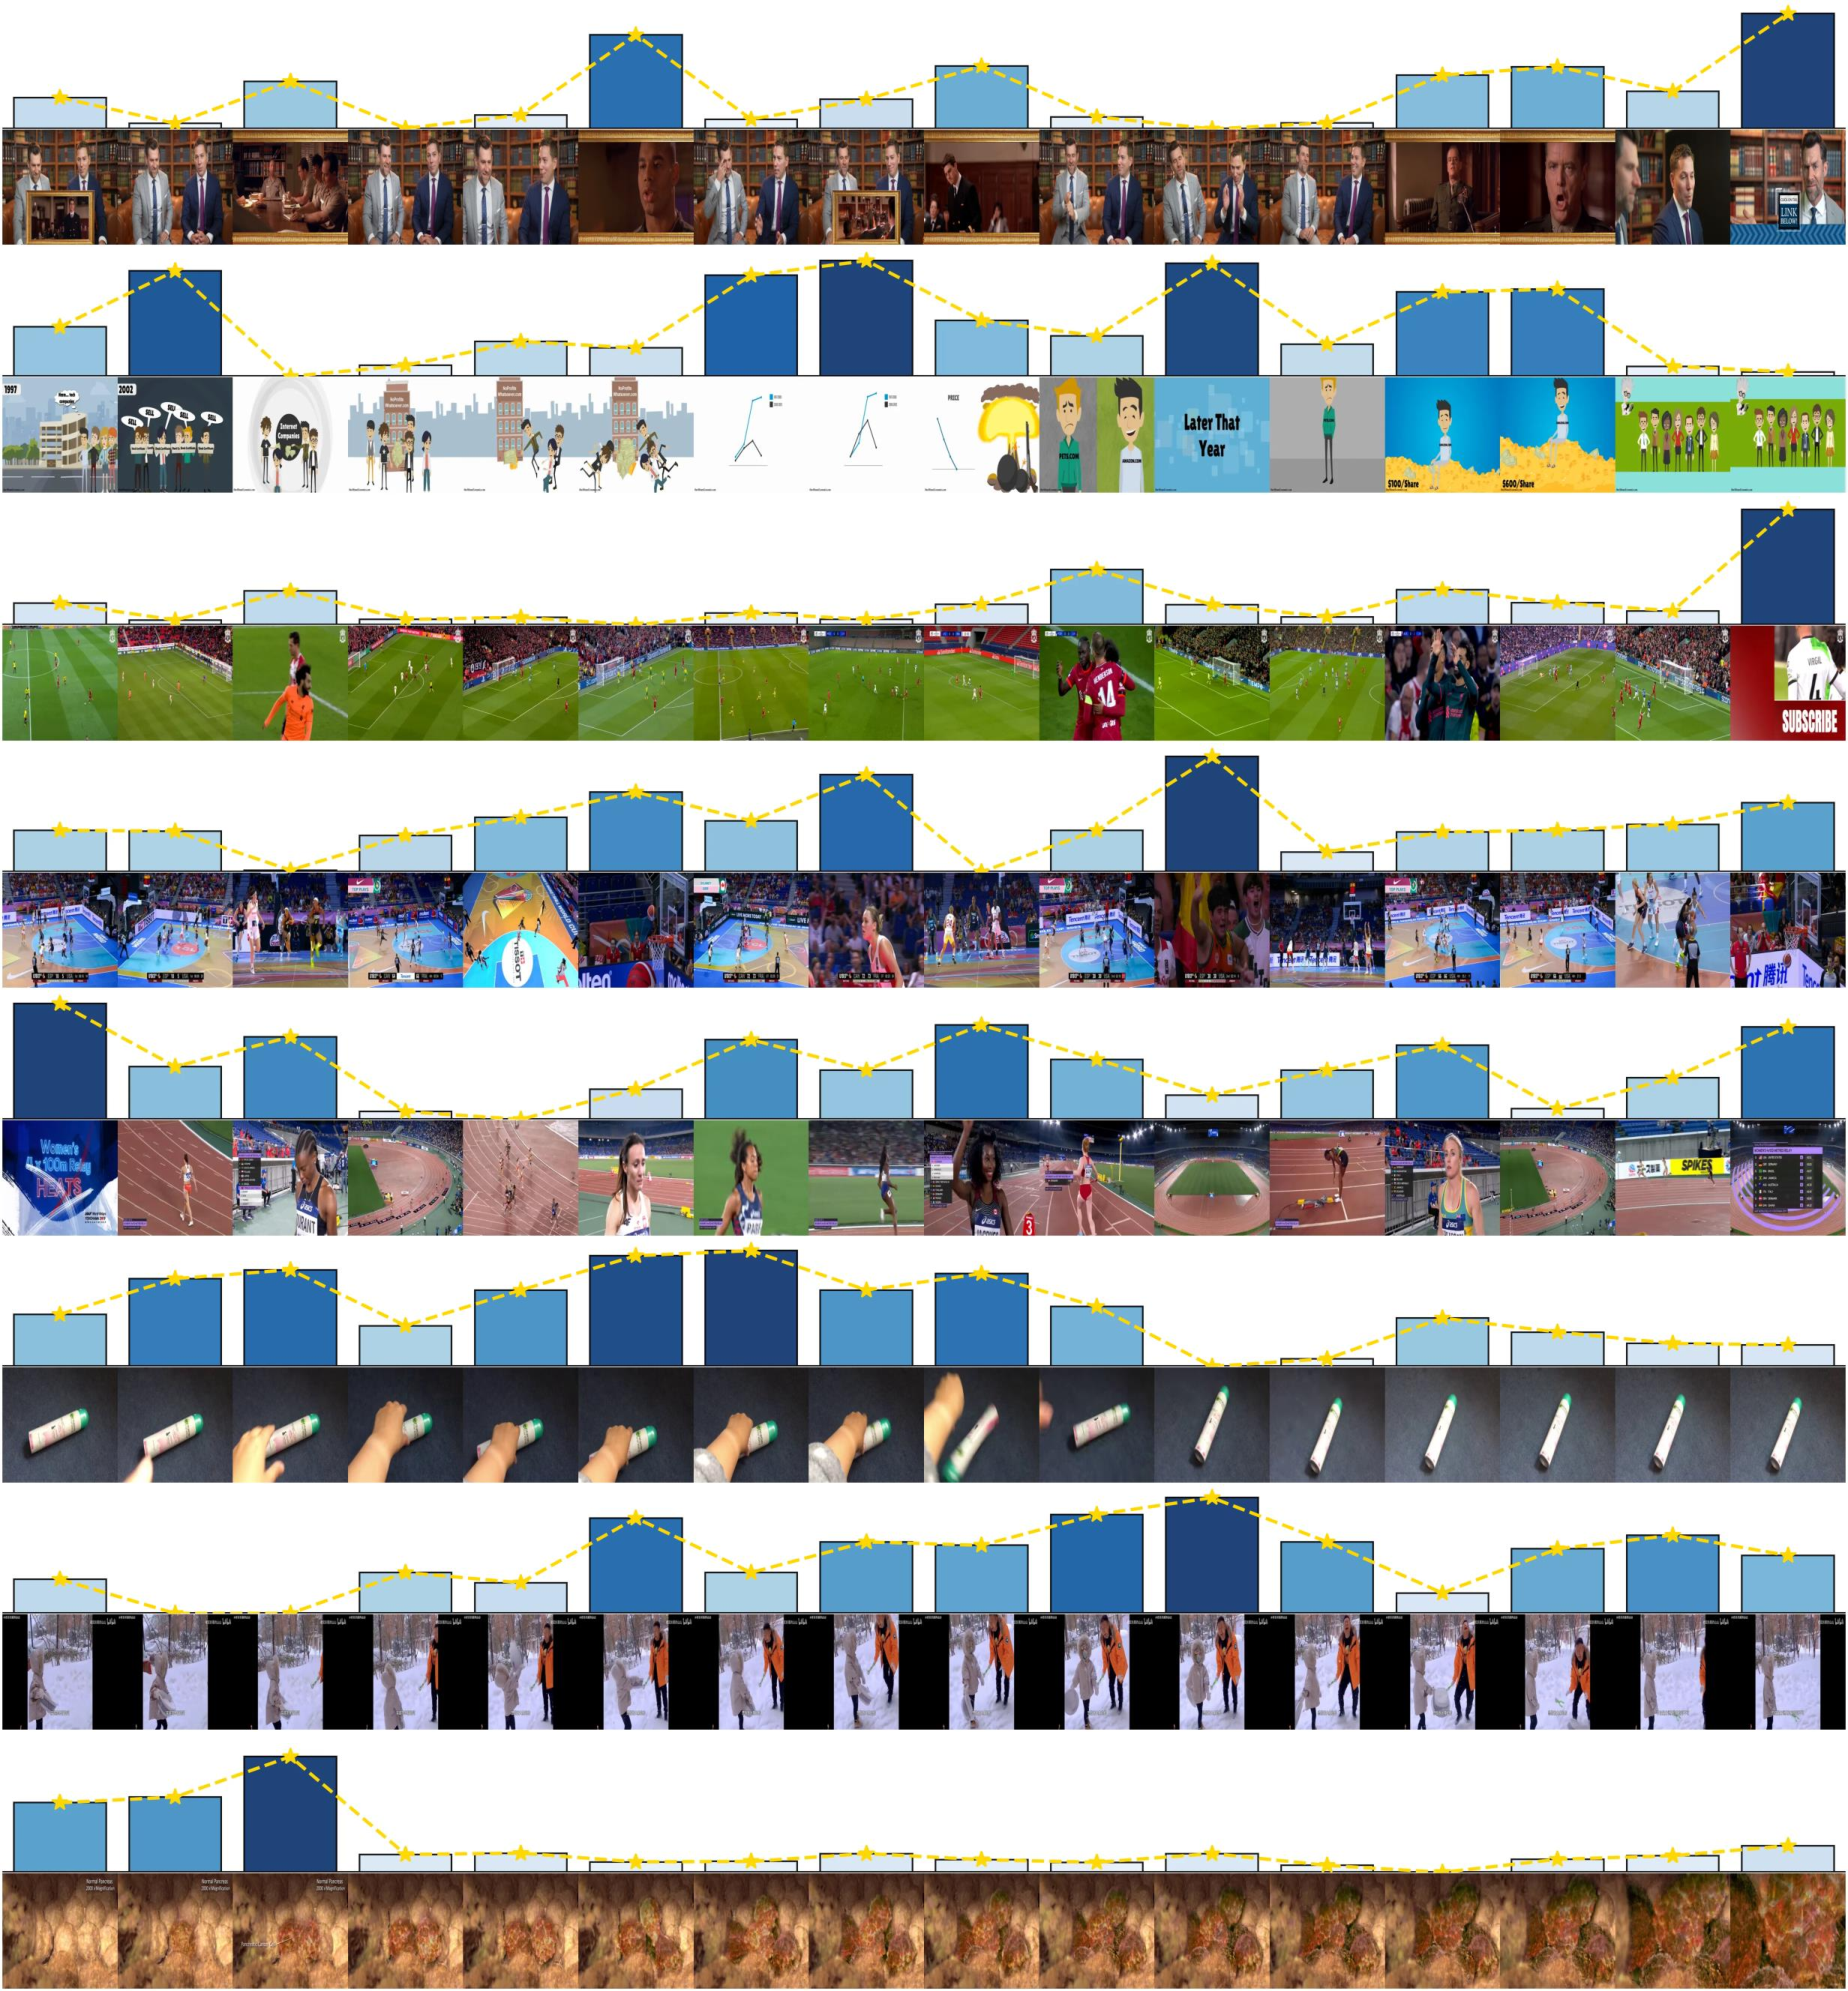
\includegraphics[width=\linewidth]{latex/figures/frame_score_vis_appendix.pdf}
   \vspace{-7mm}
    \caption{\textbf{More visualization of frame uniqueness quantified by our VidCom$^2$.} In most cases, the frame uniqueness determined by VidCom$^2$ aligns well with human video perception.}   
   \label{fig:frame_uniqueness_appendix}
   \vspace{-4mm}
\end{figure*}



